\documentclass{report}

\usepackage{booktabs}
\usepackage{copyrightbox}
\usepackage{graphics}
{% raw %}
\graphicspath{{../references/}{../results/figs}}
{% endraw %}
\usepackage{tabularx}
\usepackage{url}


\begin{document}
\title{ {{ cookiecutter.project_name }} }
\author{ {{ cookiecutter.author_name }} }
\maketitle

\begin{abstract}
{{ cookiecutter.description }}
\end{abstract}


\tableofcontents

\chapter{Overview}
\section{Naming scheme}
The \texttt{contexere} package provides tools for using an efficient naming convention for research artefacts \cite{Contexere}. 
Its command line interface is shown in Fig.~\ref{fig:cli}.
The date abbreviations for the naming scheme are summarised in Fig.~\ref{fig:date_abbreviations}.

The scheme for the identifiers of research artefact groups is \texttt{PIDyymDc[\_link[\_link]]}:
\begin{description}
\item[{\texttt{PID}}] is the project identifier  \texttt{[a-zA-Z]*} consisting of an arbitrary string of ASCII characters. 
\item[{\texttt{yy}}] is the two-digit truncated year \texttt{[0-9][0-9]} of RFC6350 \cite[p. 12]{Perreault2011_vCard} based on ISO.8601.2000 with the intention to increase information density and avoid the redundancy of slowly changing century ordinals\footnote{It can savely be assumed that project identiers \texttt{PID} change faster than the century ordinals such that any disambiguities of the truncated year will be avoided by changed \texttt{PID}s.}. 
\item[{\texttt{m}}] is one of the letters \texttt{[o-z]} encoding the month (left columns in Table~\ref{tab:date}). The month sequence \texttt{[o-z]} starts with the letter \texttt{o} because the twelve letters \texttt{opqrstuvwxyz} avoid the letter \texttt{l}, which can be easily confused with digit \texttt{1} for some fonts.
\item[{\texttt{D}}] is one of the ASCII characters \texttt{[1-9,A-V]} encoding the calendar day (columns 3--6 in Table~\ref{tab:date}). Digits 1 to 9 encode the first nine days of each months and characters \texttt{A} to \texttt{V} days 11 to 31. Digits and upper-case characters have approximately the same height, such that this element gives a visual structure to the RAG identifier, which divides the date from the daily counter.
\item[{\texttt{c}}] is one of the lower case letters \texttt{[a-z]} encoding a daily counter of research artefact groups in alphabetical order. Realistically, a typical work day won't have more than 26 different non-trivial research activities. Otherwise, there are strong indications that several closely realated research activities should be grouped together.
\item[{\texttt{link}}] is an optional abbreviation of a predecessor RAG identifier indicating the predecessar RAG contributes to the current RAG. The predecessar RAG identifier is abbreviated by showing only its last significant ASCII characters of the identifier, which are deviating from the current RAG identifier. A list of \texttt{link}s is separated by underscores with the abbreviated RAG identifiers  being listed in achronological order.
\end{description}
 

\begin{figure}
\begin{center}
\copyrightbox{
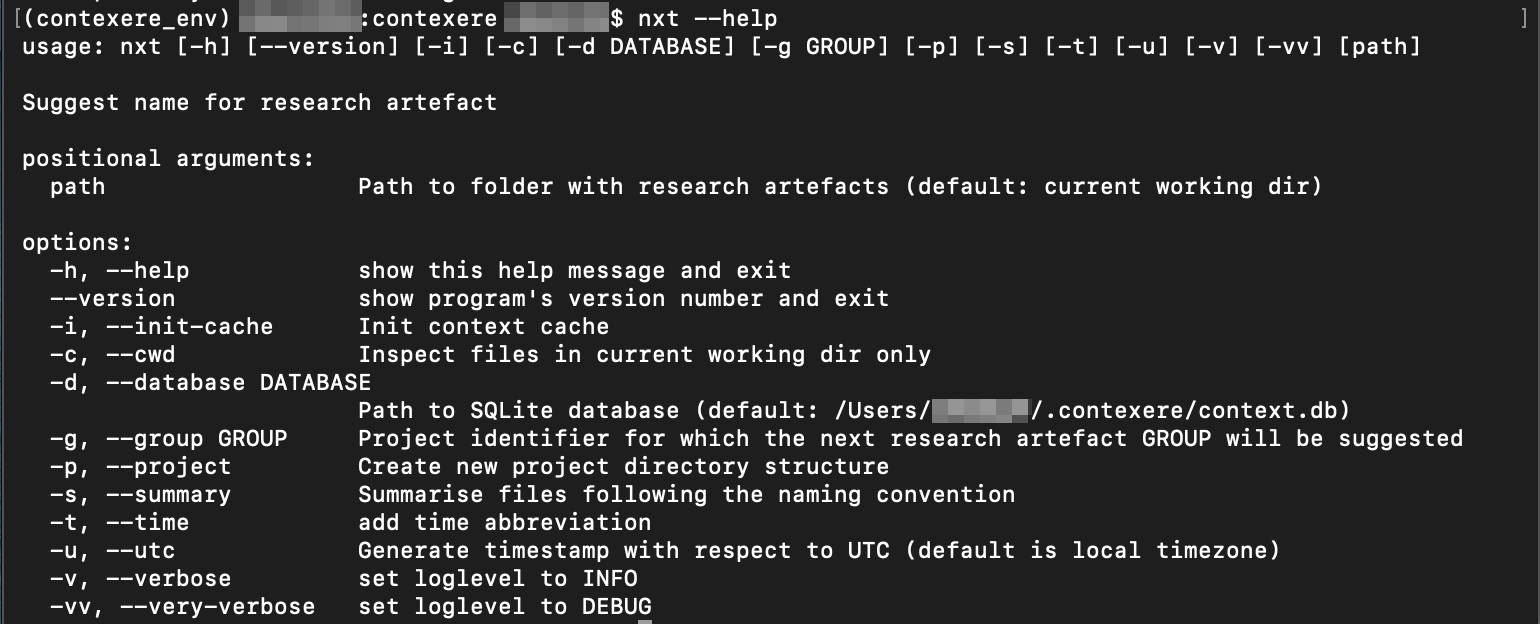
\includegraphics[width=\textwidth]{KM26qGb_a__nxt_cli.png}
}
{\texttt{KM26qGb\_a\_\_nxt\_cli.png}}
\end{center}
\caption{Command line interface of the ~nxt~ command provided by the Python package ~contexere~.}
\label{fig:cli}
\end{figure}

\begin{table}[t] 
\caption{\label{tab:date}Month and day abbreviations for research artefact groups. The month-day abbreviation \texttt{md} is appended to the truncated two-digit year abbreviation \texttt{yy} \cite[p. 12]{Perreault2011_vCard}. E.g., the code \texttt{26q1} represents the date 2026-03-01 with just four key strokes.}
\begin{tabularx}{\textwidth}{cccccccc}
  \toprule
  \multicolumn{2}{c}{Months} & \multicolumn{2}{c}{Days 1--10}
  & \multicolumn{2}{c}{Days 11-20} & \multicolumn{2}{c}{Days 21-31} \\
\texttt{m} & Month & \texttt{D} & day & \texttt{D} & day & \texttt{D} & day\\
\midrule
\texttt{o} & January & \texttt{1} & 1 & \texttt{B} & 11 & \texttt{L} & 21\\
\texttt{p} & February & \texttt{2} & 2 & \texttt{C} & 12 & \texttt{M} & 22\\
\texttt{q} & March & \texttt{3} & 3 & \texttt{D} & 13 & \texttt{N} & 23\\
\texttt{r} & April & \texttt{4} & 4 & \texttt{E} & 14 & \texttt{O} & 24\\
\texttt{s} & May & \texttt{5} & 5 & \texttt{F} & 15 & \texttt{P} & 25\\
\texttt{t} & June & \texttt{6} & 6 & \texttt{G} & 16 & \texttt{Q} & 26\\
\texttt{u} & July & \texttt{7} & 7 & \texttt{H} & 17 & \texttt{R} & 27\\
\texttt{v} & August & \texttt{8} & 8 & \texttt{I} & 18 & \texttt{S} & 28\\
\texttt{w} & September & \texttt{9} & 9 & \texttt{J} & 19 & \texttt{T} & 29\\
\texttt{x} & October & \texttt{A} & 10 & \texttt{K} & 20 & \texttt{U} & 30\\
\texttt{y} & November &  &  &  &  & \texttt{V} & 31\\
\texttt{z} & December &  &  &  &  &  & \\
\bottomrule
\end{tabularx}
\end{table}

{% raw %}
\bibliographystyle{plain} % 
\bibliography{{../references/{% endraw %}{{ cookiecutter.repo_name }}{% raw %}_bibliography}}

\end{document}
{% endraw %}